\chapter{Introducción específica} % Main chapter title

\label{Chapter2}

%----------------------------------------------------------------------------------------
%	SECTION 1
%----------------------------------------------------------------------------------------
%Todos los capítulos deben comenzar con un breve párrafo introductorio que indique cuál es el contenido que se encontrará al leerlo.  La redacción sobre el contenido de la memoria debe hacerse en presente y todo lo referido al proyecto en pasado, siempre de modo impersonal.
En este capítulo se abordarán temas referentes al análisis de la estructura del sistema que se desarrolló, gestión, planificación del trabajo y técnicas relacionadas al sensor empleado.  	 

\section{Estructura general del sistema}
\label{sec:estructgeneralsistema}

%\subsection{Uso de mayúscula inicial para los título de secciones}

%Si en el texto se hace alusión a diferentes partes del trabajo referirse a ellas como capítulo, sección o subsección según corresponda. Por ejemplo: ``En el capítulo \ref{Chapter1} se explica tal cosa'', o ``En la sección \ref{sec:ejemplo} se presenta lo que sea'', o ``En la subsección \ref{subsec:ejemplo} se discute otra cosa''.
 
Con el avance del diseño de un plano para la fabricación del prototipo para los diferentes ensayos a realizar, y con el método de aforo por compuerta a utilizar para la medición de caudal, ligeramente se identificó que emplear una compuerta se generarían filtraciones de agua en sus guías de desplazamiento que, en una maqueta, a escala producirían errores considerables al momento de realizar las mediciones relacionadas a la altura de la superficie de agua, y cálculos pertinentes para determinar el caudal, por lo que en el sistema no se obtendrían los resultados esperados. En este entorno, el flujo de agua que fluya por debajo de la compuerta sería menor que en el caudalímetro, instrumento ubicado en un punto distante de la compuerta en el sentido que fluye el recurso hídrico. De esta forma, obtendríamos dos valores de caudales diferentes debido, entre otros factores, a las filtraciones.     
Esto motivo reemplazar, en el prototipo, la compuerta por una válvula y así eliminar los errores que introducen dichas filtraciones. 
Para el control de la válvula se elaboró un servomotor con el empleo de un motor paso a paso con su correspondiente controlador.
\begin{figure}[h]
\centering
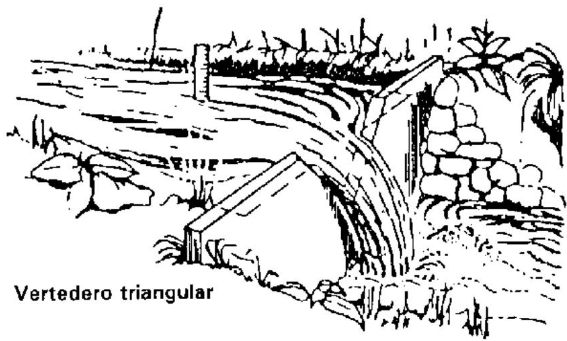
\includegraphics[scale=.50]{./Figures/VertederoTriangular.png}
\caption{Ilustración de un vertedero triangular ubicado en determinado punto a medir caudal en el canal.}
\end{figure}

Para medir el caudal, se fabricó un caudalímetro por placa de aforo triangular. Estos tipos de instrumentos, también denominados vertederos, representan un dique o pared que intercepta en un determinado punto una corriente de liquido, en este caso agua, con superficie libre, como se puede apreciar en la "Figura 2.1" . En general, se utilizan para mantener un nivel de superficie de aguas arriba que no exceda de un valor limite, o bien para medir el caudal de agua circulante por un canal. Este instrumento resulta un medidor de caudal sencillo pero efectivo en canales abiertos. 

%El principio de funcionamiento del módulo patrón en el prototipo a escala consiste: mediante un firmware controlar el eje de un servomotor, que por medio de un mecanizado entre dicho servomotor y una válvula, dominar el movimiento de esta última y así establecer el caudal de agua en el valor que desea fijar el usuario.
El principio de funcionamiento de la celda primaria, en el prototipo a escala, consiste en el control del eje de un servomotor, que por medio de un mecanizado entre dicho servomotor y una válvula, domina el movimiento de esta última y así establece el caudal de agua en el valor que desea fijar el usuario.

El diagrama de control correspondiente es el que se muestra en la "Figura \ref{fig:CeldaPrimaria}". La salida del servomotor actúa directamente sobre la válvula, que en este caso es una llave esférica, pero podría ser sin ningún inconveniente un sistema de cremallera para abrir una compuerta vertical, como las que podemos encontrar con reiteración en los canales de agua a cielo abierto. La salida de la válvula es el flujo controlado de caudal al canal, en este punto se coloca un medidor de caudal que luego su resultado es comparado con el set point, el cual es un valor de caudal fijado por el usuario. En el sumador, la diferencia que existe entre el set point y el valor de caudal medido se obtiene una señal de error, que luego es procesada por un algoritmo de control PID para que la misma sea cero.


%En el sistema correspondiente al modulo patrón, se detectó la necesidad de realimentar una señal correspondiente a un sensor de presión el cual brinda cierta información de la cual podemos identificar, mediante un proceso de cálculos matemático, el nivel de altura de la superficie del agua. Este sensor de presión se encuentra ubicado muy próximo, en el orden de los milímetros, del caudalímetro. Esta señal, proveniente del sensor, es inyectada al firmware no solo para identificar el nivel del agua, sino también para obtener un valor estimado de caudal de agua que circula a través del caudalímetro, y de esta forma regular el caudal de agua controlando el movimiento del servomotor-válvula.
%Este funcionamiento interno del Sistema-Módulo Patrón se representa mediante un diagrama en bloques en la siguiente "Figura \ref{fig:MóduloPatrón}".
%  
\begin{figure}[h]
\centering
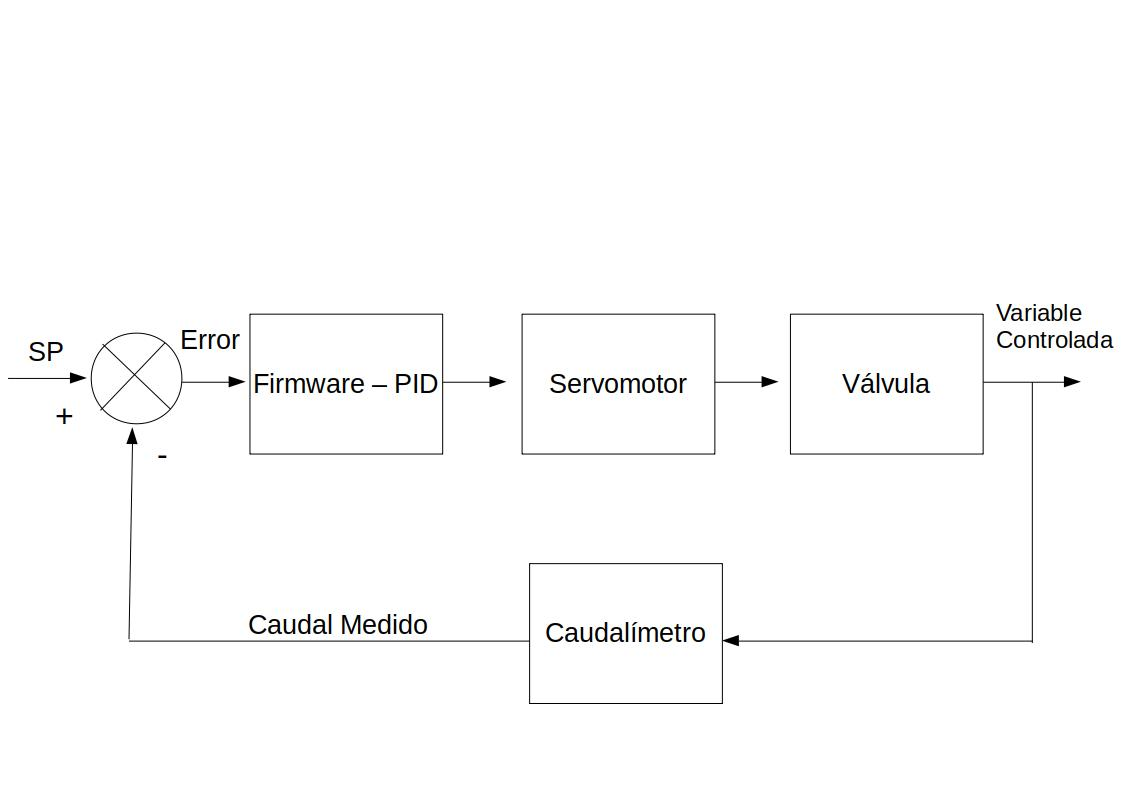
\includegraphics[scale=.45]{./Figures/DiagramaEnBloqueDeControlCeldaPrimaria-V4.jpg}
\caption{Diagrama en bloque de control - celda primaria.}
\label{fig:CeldaPrimaria}
\end{figure}

\section{Compuertas miller}
\label{sec:ejemplo}
Las compuertas Miller es el mecanismo más utilizado en los canales de agua de riego para controlar la entrada de agua de los canales ramales y tomas directas a las parcelas. Están construidas de fierro fundido (vaciado o colado) por su resistencia a la oxidación; sin embargo, son frágiles y poco maleables. La toma Miller, en esencia, es una compuerta circular que obtura la entrada a la tubería de salida, la que es izada por un mecanismo elevador compuesto de un vástago cilíndrico con cuerda tipo tornillo (roscas), generalmente de 2” de diámetro y longitud variable, en función de la altura a colocar la toma y un volante. Las tomas-granja Miller se clasifican por el diámetro de la tubería a obturar, y son de 18” y 24” las más comunes para tomas-granjas, mientras que las de 30” y 36” son usadas para abastecer ramales y subramales.
Las ventajas de este tipo de tomas es que son relativamente baratas, la mayoría de las fundidoras las pueden construir y son de fácil colocación. Como desventajas, destacan que pueden tener filtraciones de consideración al ser difícil un cierre hermético debido al metal de la tubería y de la compuerta (comal), especialmente si, durante su fundición, no hay cuidado de tener acabados completamente a nivel. La calibración de esta estructura es difícil, ya que al abrirse parcialmente la compuerta circular sobre la tubería circular, se forman secciones tipo “media luna” con área hidráulica variable, sin seguir un patrón de fácil cálculo.

\begin{figure}[h]
\centering
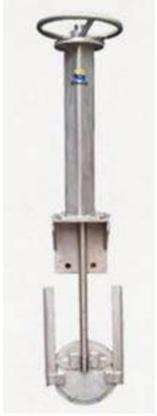
\includegraphics[scale=.55]{./Figures/CompuertaMiller.jpeg}
\caption{Compuerta tipo miller para toma-granja.}
\label{fig:CeldaPrimaria}
\end{figure}

\begin{figure}[h]
\centering
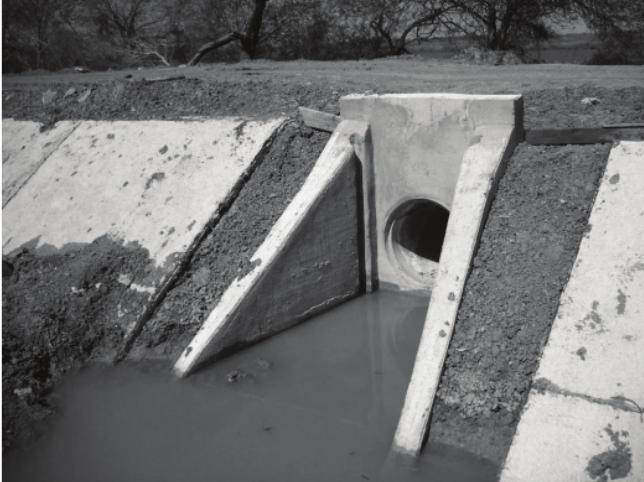
\includegraphics[scale=.55]{./Figures/ConductoPreparadoParaCompuertaMiller.jpeg}
\caption{Conducto preparado para colocar compuerta tipo miller.}
\label{fig:CeldaPrimaria}
\end{figure}

\begin{figure}[h]
\centering
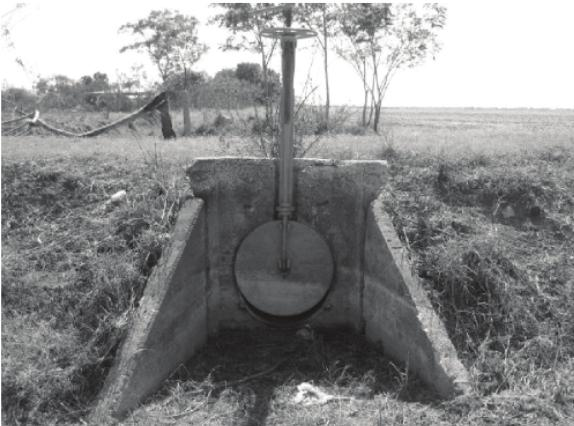
\includegraphics[scale=.55]{./Figures/compuertamillercircular.jpeg}
\caption{Toma-granja tipo miller de compuerta circular de 18” de diámetro.}
\label{fig:CeldaPrimaria}
\end{figure}

Este mecanismo que se mostró y que se emplea en muchos países para el control de entrada de agua a los canales principales o bien a las parcelas, impulso a utilizar, en el prototipo a escala, una válvula esférica simulando ser una compuerta miller.   

\section{Especificación del Software y Hardware}
\label{sec:ejemplo}
A continuación se presentan los requerimientos específicos de software y hardware del sistema, que se tuvieron en cuenta al momento de inicio del desarrollo de este proyecto, cuyo fin es, mediante el control de movimiento de una válvula regular el caudal de agua según las necesidades del usuario. 
\subsection{Requisitos específicos del software}
\label{subsec:ejemplo}


 Los requisitos específicos de software fueron:

\begin{enumerate}
	\item El firmware deberá generar como señal, trenes de pulsos para controlar el movimiento del eje perteneciente al servomotor.
	\item El firmware deberá determinar, mediante el sensor  de presión en conjunto con el caudalímetro por placa de aforo triangular, el caudal de agua que fluye a través de este instrumento de medición.
	\item  El firmware deberá incluir un algoritmo de control PID, que por medio de un lazo de retroalimentación permita regular la variable a controlar.
	\item El firmware deberá ser capaz, a través de un pin configurado como salida, establecer el sentido de giro del eje del servomotor, horario - antihorario.
	\item El firmware deberá ser capaz, a través de un pin configurado como salida, habilitar - deshabilitar el servomotor.
	\item El firmware deberá interactuar, mediante el empleo del puerto serial, con otra aplicación. 	  
	\item Con un protocolo de comunicación definido entre la aplicación externa y el firmware, este último deberá ser capaz de recibir y enviar datos.
	\item El firmware deberá enviar una notificación de correcta recepción de cualquier comando mediante el envío de un comando específico hacía la aplicación externa.  
	\item El firmware deberá reportar o notificar a la aplicación externa la recepción de un comando inválido mediante un comando específico.
	\item En caso de recepción de comandos válidos, el firmware deberá informar internamente que hay datos a procesar. 
\end{enumerate}

\subsection{Requisitos específicos del hardware}
\label{subsec:requisitoshw}
 Los requisitos específicos principales de hardware fueron:
\begin{enumerate}
	\item Se hará uso de la placa EDU-CIAA-NXP como computadora principal para el prototipo a escala.
	\item Se construirá un mecanizado de  válvula de control estándar mediante un servomotor energizado paso a paso y un elemento medidor de ángulo tipo potenciométrico resistivo.
	\item Se construirá un medidor de caudal por canal de aforo utilizando para la medición de la altura de nivel de agua un sensor MPX5010DP.
	\item Se diseñará y fabricará un circuito como interfaz que controlará las señales enviadas desde la placa EDU-CIAA-NXP al controlador del servomotor paso a paso. 
\end{enumerate}

\section{Planificación}
\label{sec:planificacion}
La planificación original presentada al iniciar el proyecto contemplaba un trabajo de 600 horas. Los atrasos relacionados con la problemática identificada y expuesta en la sección \ref{sec:estructgeneralsistema}, significó repensar un nuevo prototipo con una válvula de control  mecanizada. Esto, implicó recurrir a una empresa dedicada a la mecanización de piezas para adaptar el servomotor y una válvula esférica. Como consecuencia de esto, no se pudo contar en tiempo y forma con la pieza total, por lo que se tuvo que modificar la planificación inicial. 
A continuación, se presenta la tabla \ref{tab:seccplanificacion}, la misma detalla el desglose de tareas pertinente a la planificación original. 
\begin{table}[h]
	\centering
	\caption[caption corto]{Desglose de tareas}
	\begin{tabular}{l c c}    
		\toprule
		\textbf{WBS}  & \textbf{Tareas} 	 & \textbf{Tiempo[hs]}\\
		\midrule
		1.   & Documentación y Análisis Preliminar	&  19 \\		
		1.1  & Planificación del proyecto			&  24 \\
		1.2  & Análisis de bibliográfica especifica &  20 \\
		1.3  & Definición de casos de pruebas		&  15 \\
		2.   & Investigación, Diseño e Implementación & 127 \\
		2.1  & Inicialización del entorno de trabajo  & 34\\
		2.2  & Investigación y diseño del circuito controlador del motor & 12\\
		2.3 & Investigación y diseño del circuito para el sensor lineal &31\\
		2.4 & Definición de la arquitectura del firmware & 54\\
		2.5 & Definición de las interfaces y API’s  &32\\
		2.6 & Implementación de módulo controlador de motor &15\\
		2.7 & Implementación de módulos de adquisición de datos &12\\
		2.8 & Implementación de módulo de comunicación & 16\\
		2.9 & Implementación de herramientas de testing & 18\\
		2.10 & Integración de módulos & 21\\
		2.11 & Investigación  del sensor de presión diferencial & 15\\
		2.12 & Calibración del sensor de presión diferencial y diseño del circuito &13\\
		3. & Verificación y Validación & 48\\
		3.1 & Pruebas unitarias en submódulos &24\\
		3.2 & Pruebas de integración &19\\
		3.3 & Pruebas de Sistema &23\\
		4. & Cierre & 36\\
		4.1 & Elaboración del Informe del proyecto & 24\\
		4.2 & Elaboración de presentación final del proyecto &12\\
		\bottomrule
		\hline
	\end{tabular}
	\label{tab:seccplanificacion}
\end{table}

%Cuando se quiere poner una lista tabulada, se hace así:
%
%\begin{itemize}
%	\item Este es el primer elemento de la lista.
%	\item Este es el segundo elemento de la lista.
%\end{itemize}
%
%Notar el uso de las mayúsculas y el punto al final de cada elemento.
%
%Si se desea poner una lista numerada el formato es este:
%
%\begin{enumerate}
%	\item Este es el primer elemento de la lista.
%	\item Este es el segundo elemento de la lista.
%\end{enumerate}
%
%Notar el uso de las mayúsculas y el punto al final de cada elemento.
%
%\subsection{Este es el título de una subsección}
%\label{subsec:ejemplo}
%
%Se recomienda no utilizar \textbf{texto en negritas} en ningún párrafo, ni tampoco texto \underline{subrayado}. En cambio sí se debe utilizar \textit{texto en itálicas} para palabras en un idioma extranjero, al menos la primera vez que aparecen en el texto. En el caso de palabras que estamos inventando se deben utilizar ``comillas'', así como también para citas textuales. Por ejemplo, un \textit{digital filter} es una especie de ``selector'' que permite separar ciertos componentes armónicos en particular.
%
%La escritura debe ser impersonal. Por ejemplo, no utilizar ``el diseño del firmware lo hice de acuerdo con tal principio'', sino ``el firmware fue diseñado utilizando tal principio''. 
%
%El trabajo es algo que al momento de escribir la memoria se supone que ya está concluido, entonces todo lo que se refiera a hacer el trabajo se narra en tiempo pasado, porque es algo que ya ocurrió. Por ejemplo, "se diseñó el firmware empleando la técnica de test driven development".
%
%En cambio, la memoria es algo que está vivo cada vez que el lector la lee. Por eso transcurre siempre en tiempo presente, como por ejemplo:
%
%``En el presente capítulo se da una visión global sobre las distintas pruebas realizadas y los resultados obtenidos. Se explica el modo en que fueron llevados a cabo los test unitarios y las pruebas del sistema''.
%
%Se recomienda no utilizar una sección de glosario sino colocar la descripción de las abreviaturas como parte del mismo cuerpo del texto. Por ejemplo, RTOS (\textit{Real Time Operating System}, Sistema Operativo de Tiempo Real) o en caso de considerarlo apropiado mediante notas a pie de página.
%
%Si se desea indicar alguna página web utilizar el siguiente formato de referencias bibliográficas, dónde las referencias se detallan en la sección de bibliografía de la memoria, utilizado el formato establecido por IEEE en \citep{IEEE:citation}. Por ejemplo, ``el presente trabajo se basa en la plataforma EDU-CIAA-NXP \citep{CIAA}, la cual...''.
%
%\subsection{Figuras} 
%
%Al insertar figuras en la memoria se deben considerar determinadas pautas. Para empezar, usar siempre tipografía claramente legible. Luego, tener claro que \textbf{es incorrecto} escribir por ejemplo esto: ``El diseño elegido es un cuadrado, como se ve en la siguiente figura:''
%
%\begin{figure}[h]
%\centering
%
\includegraphics[scale=.50]{./Figures/cuadradoAzul.png}
%\end{figure}
%
%La forma correcta de utilizar una figura es con referencias cruzadas, por ejemplo: ``Se eligió utilizar un cuadrado azul para el logo, como puede observarse en la figura \ref{fig:cuadradoAzul}''.
%
%\begin{figure}[ht]
%	\centering
%	
\includegraphics[scale=.45]{./Figures/cuadradoAzul.png}
%	\caption{Ilustración del cuadrado azul que se eligió para el diseño del logo.}
%	\label{fig:cuadradoAzul}
%\end{figure}
%
%El texto de las figuras debe estar siempre en español, excepto que se decida reproducir una figura original tomada de alguna referencia. En ese caso la referencia de la cual se tomó la figura debe ser indicada en el epígrafe de la figura e incluida como una nota al pie, como se ilustra en la figura \ref{fig:palabraIngles}.
%
%\begin{figure}[htpb]
%	\centering
%	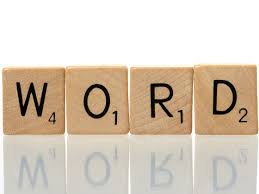
\includegraphics[scale=.3]{./Figures/word.jpeg}
%	\caption{Imagen tomada de la página oficial del procesador\protect\footnotemark.}
%	\label{fig:palabraIngles}
%\end{figure}
%
%\footnotetext{Imagen tomada de \url{https://goo.gl/images/i7C70w}}
%
%La figura y el epígrafe deben conformar una unidad cuyo significado principal pueda ser comprendido por el lector sin necesidad de leer el cuerpo central de la memoria. Para eso es necesario que el epígrafe sea todo lo detallado que corresponda y si en la figura se utilizan abreviaturas entonces aclarar su significado en el epígrafe o en la misma figura.
%
%
%
%\begin{figure}[ht]
%	\centering
%	
\includegraphics[scale=.37]{./Figures/questionMark.png}
%	\caption{¿Por qué de pronto aparece esta figura?}
%	\label{fig:questionMark}
%\end{figure}
%
%Nunca colocar una figura en el documento antes de hacer la primera referencia a ella, como se ilustra con la figura \ref{fig:questionMark}, porque sino el lector no comprenderá por qué de pronto aparece la figura en el documento, lo que distraerá su atención.
%
%Otra posibilidad es utilizar el entorno \textit{subfigure} para incluir más de una figura, como se puede ver en la figura \ref{fig:three graphs}. Notar que se pueden referenciar también las figuras internas individualmente de esta manera: \ref{fig:1de3}, \ref{fig:2de3} y \ref{fig:3de3}.
% 
%\begin{figure}[!htpb]
%     \centering
%     \begin{subfigure}[b]{0.3\textwidth}
%         \centering
%         
\includegraphics[width=.65\textwidth]{./Figures/questionMark}
%         \caption{Un caption.}
%         \label{fig:1de3}
%     \end{subfigure}
%     \hfill
%     \begin{subfigure}[b]{0.3\textwidth}
%         \centering
%         
\includegraphics[width=.65\textwidth]{./Figures/questionMark}
%         \caption{Otro.}
%         \label{fig:2de3}
%     \end{subfigure}
%     \hfill
%     \begin{subfigure}[b]{0.3\textwidth}
%         \centering
%         
\includegraphics[width=.65\textwidth]{./Figures/questionMark}
%         \caption{Y otro más.}
%         \label{fig:3de3}
%     \end{subfigure}
%        \caption{Tres gráficos simples}
%        \label{fig:three graphs}
%\end{figure}
%
%El código para generar las imágenes se encuentra disponible para su reutilización en el archivo \file{Chapter2.tex}.
%
%\subsection{Tablas}
%
%Para las tablas utilizar el mismo formato que para las figuras, sólo que el epígrafe se debe colocar arriba de la tabla, como se ilustra en la tabla \ref{tab:peces}. Observar que sólo algunas filas van con líneas visibles y notar el uso de las negritas para los encabezados.  La referencia se logra utilizando el comando \verb|\ref{<label>}| donde label debe estar definida dentro del entorno de la tabla.
%
%\begin{verbatim}
%\begin{table}[h]
%	\centering
%	\caption[caption corto]{caption largo más descriptivo}
%	\begin{tabular}{l c c}    
%		\toprule
%		\textbf{Especie}     & \textbf{Tamaño} & \textbf{Valor}\\
%		\midrule
%		Amphiprion Ocellaris & 10 cm           & \$ 6.000 \\		
%		Hepatus Blue Tang    & 15 cm           & \$ 7.000 \\
%		Zebrasoma Xanthurus  & 12 cm           & \$ 6.800 \\
%		\bottomrule
%		\hline
%	\end{tabular}
%	\label{tab:peces}
%\end{table}
%\end{verbatim}
%
%
%\begin{table}[h]
%	\centering
%	\caption[caption corto]{caption largo más descriptivo}
%	\begin{tabular}{l c c}    
%		\toprule
%		\textbf{Especie} 	 & \textbf{Tamaño} 		& \textbf{Valor}  \\
%		\midrule
%		Amphiprion Ocellaris & 10 cm 				& \$ 6.000 \\		
%		Hepatus Blue Tang	 & 15 cm				& \$ 7.000 \\
%		Zebrasoma Xanthurus	 & 12 cm				& \$ 6.800 \\
%		\bottomrule
%		\hline
%	\end{tabular}
%	\label{tab:peces}
%\end{table}
%
%En cada capítulo se debe reiniciar el número de conteo de las figuras y las tablas, por ejemplo, figura 2.1 o tabla 2.1, pero no se debe reiniciar el conteo en cada sección. Por suerte la plantilla se encarga de esto por nosotros.
%
%\subsection{Ecuaciones}
%\label{sec:Ecuaciones}
%
%Al insertar ecuaciones en la memoria dentro de un entorno \textit{equation}, éstas se numeran en forma automática  y se pueden referir al igual que como se hace con las figuras y tablas, por ejemplo ver la ecuación \ref{eq:metric}.
%
%\begin{equation}
%	\label{eq:metric}
%	ds^2 = c^2 dt^2 \left( \frac{d\sigma^2}{1-k\sigma^2} + \sigma^2\left[ d\theta^2 + \sin^2\theta d\phi^2 \right] \right)
%\end{equation}
%                                                        
%Es importante tener presente que si bien las ecuaciones pueden ser referidas por su número, también es correcto utilizar los dos puntos, como por ejemplo ``la expresión matemática que describe este comportamiento es la siguiente:''
%
%\begin{equation}
%	\label{eq:schrodinger}
%	\frac{\hbar^2}{2m}\nabla^2\Psi + V(\mathbf{r})\Psi = -i\hbar \frac{\partial\Psi}{\partial t}
%\end{equation}
%
%Para generar la ecuación \ref{eq:metric} se utilizó el siguiente código:
%
%\begin{verbatim}
%\begin{equation}
%	\label{eq:metric}
%	ds^2 = c^2 dt^2 \left( \frac{d\sigma^2}{1-k\sigma^2} + 
%	\sigma^2\left[ d\theta^2 + 
%	\sin^2\theta d\phi^2 \right] \right)
%\end{equation}
%\end{verbatim}
%
%Y para la ecuación \ref{eq:schrodinger}:
%
%\begin{verbatim}
%\begin{equation}
%	\label{eq:schrodinger}
%	\frac{\hbar^2}{2m}\nabla^2\Psi + V(\mathbf{r})\Psi = 
%	-i\hbar \frac{\partial\Psi}{\partial t}
%\end{equation}
%
%\end{verbatim}